%!TEX root = ../Thesis.tex

\chapter{Metodología}\label{ch:chap5}

\epigraphhead[70]{
\epigraph{There was nowhere to go but everywhere, so just keep on rolling under the stars.}
{Jack Kerouac}}

A continuación se describe la metodología que se llevó a cabo para la tarea de \sd. 

Como ya se describió en el \autoref{ch:chap2} es necesaria una etapa de pre-procesamiento en el sistema; primero para eliminar de la señal de audio las cosas que no nos interesan (que en este caso son silencios), para lo que se usó un detector de energía y así ignorar los instantes en los que ningún interlocutor participa. 

Luego, también en la etapa de pre-procesamiento se encuentra el obtener vectores de características que representen de alguna manera la señal, y que sean mucho más fáciles de manipular. Para esta etapa se usaron los \ac{MFCC}, siguiendo el \autoref{alg:mfcc}.  Después de obtener los vectores característicos, se agruparon mediante k-means++ (\autoref{alg:kmeanspp}) para de alguna forma discretizar todas las posibles palabras emitidas en el diálogo. Esta agrupación inicial nos permitirá reducir la dimensionalidad de los vectores, así como aglomerar aquellos que sean muy similares con respecto a los demás.

Después de esta etapa de clasificación, ya se tendrán los datos como observaciones que representarán las variables observadas del \ac{HMM}. Como se desconoce tal cual el número de personas involucradas en la grabación, se propondrán varios modelos $\mc{M}_d$ con $d$ estados ocultos. El valor de $d$ variará de acuerdo a qué tan extensas se deseen hacer las pruebas, pero a priori no hay un límite pre-establecido. 

Luego, corresponderá usar el algoritmo \ac{EM} con cada uno de los modelos $\mc{M}_d$ propuestos, tanto para estimar sus parámetros como para estimar su verosimilitud. Como ya se mencionó en \autoref{ch:chap4} esta etapa se realizará varias veces, para evitar el estancamiento del método y obtener un buen ajuste del modelo. Del modelo con mayor versomilitud se calculará la segmentación correspondiente, y se almacenará. 

Después, seguirá la etapa de selección de modelo. Este proceso se realizará en dos partes: primero, explorando todo el espacio de soluciones y reduciendo los posibles modelos ganadores; y luego, seleccionando de entre los candidatos resultantes al mejor modelo.

En un primero paso, se estimará \ac{BIC} para todos los \ac{HMM} propuestos para generar una curva de selección. Como se verá en las pruebas, es necesario introducir un término de regularización en \ac{BIC} para que la penalización del modelo corresponda con las log-verosimilitudes obtenidas. 

Esto se puede hacer de la siguiente forma: 
\begin{equation}
BIC_{\lambda}(\mc{M}) = 2 \mc{L}_{max}(\mc{M}) - \lambda \cdot log N \cdot dim(M)
\end{equation}
aunque presenta el inconveniente de tener que encontrar el valor adecuado para $\lambda$ que penalice de buena forma los modelos. 

Para escoger el valor adecuado de $\lambda$ se realizará un análisis de sensibilidad, generando múltiples curvas de selección \ac{BIC} con diferentes valores de $\lambda$. Tanto la discretización como los rangos de $\lambda$ permitirán hacer una mejor búsqueda del parámetro. Con todas estas diferentes curvas, se tendrá una superficie, en donde en un eje variará el número de interlocutores del modelo, mientras que en el otro será el valor de regularización $\lambda$ el que cambiará. 

Se busca mediante este análisis encontrar la región de inflexión que divide a la superficie en dos: en la primera parte de la superficie, el valor de $\lambda$ será pequeño, por lo que siempre tendrán una mayor verosimilitud los modelos con más parámetros; mientras que en la segunda parte, la penalización sera muy grande, y se escogerán siempre los modelos más sencillos, sin darle tomar en cuenta su verosimilitud.

Por esto mismo, se puede calcular el gradiente de la superficie generada por las funciones \ac{BIC}, y se buscará la región el valor de $\lambda$ en el que la suma de los valores absolutos sea menor. 

Es importante recordar que el modelo \ac{HMM} al ser resuelto usando \ac{EM} buscará siempre maximizar la función de verosimilitud; por lo que es natural que mientras más parámetros tenga un modelo, mejor será su ajuste a los datos y mayor su verosimilitud.

Basándonos en esto, si se comparan distintos modelos con un $\lambda$ pequeño, se espera que los modelos más complejos sean los que tengan un valor \ac{BIC} mayor; por lo que habrá un gradiente en esa dirección con pendiente positiva. Por otro lado, cuando el $\lambda$ sea demasiado grande, los modelos más sencillos seran los que tengan asociado un valor de \ac{BIC} mayor; y entonces el gradiente estará en el otro sentido, con una pendiente negativa. 

El caso que nos interesa es cuando el valor de $\lambda$ penaliza de forma correcta, es decir, está en el mismo orden de magnitud que la mayoría de las verosimilitudes de los modelos. En ese momento, el gradiente de la superficie deberá tener dos direcciones, pues el valor máximo de \ac{BIC} no corresponderá al modelo más simple o al más complicado. Y además, la suma de los gradientes para ese valor será menor con respecto a otros valores de $\lambda$. 

Una vez que se logre seleccionar el $\lambda$ adecuado de regularización, se procede a evaluar su curva \ac{BIC} asociada y de ahí se obtiene al modelo ganador o un subconjunto de posibles ganadores (en caso de que varios modelos tengan puntuaciones similares de acuerdo a \ac{BIC}).

Como ya se mencionó, en el segundo paso, se realizará un proceso de refinamiento en caso de que se tengan varios modelos posibles. Para esto, se formarán pares de modelos que se deseen comparar, y se estimará su \ac{LLR}, que se denominará como $LLR_{obs}$. Para este mismo par de modelos, y mediante bootstrap paramétrico se hará una prueba de hipótesis para comproar cuál modelo es más adecuado para los datos.

Esto es, a partir de los dos modelos a examinar, se simularán múltiples secuencias de datos con los parámetros que se estimaron para cada modelo; y luego, con los datos simulados se estimará su máxima verosimilitud, para luego calcular el \ac{LLR}, que ahora se denominará $LLR_{boot}$. 

Como esta simulación se harán muchas réplicas, y con todos los valores $LLR_{boot}$ que se obtengan se formará una curva. Mediante una prueba de hipótesis se revisará si el $LLR_{obs}$ tiene la misma distribución que la curva de $LLR_{boot}$. La hipótesis nula corresponderá a que el primer modelo sea el correcto, y entonces tanto $LLR_{boot}$ como $LLR_{obs}$ tengan la misma distribución. Por otro lado, la hipótesis alternativa significaría que se rechaza $LLR_{obs}$ como una muestra de $LLR_{boot}$ bajo una significancia dada; y entonces se rechaza que el primer modelo sea el correcto.

De esta forma, se pueden realizar pruebas de hipótesis para los modelos candidatos, e ir rechazando modelos de acuerdo al análisis propuesto. En el \autoref{ch:chap6} se describe más a detalle esta selección de moledo, con las pruebas realizadas.

\section{Esquema general} 

El esquema general con las diferentes etapas que se realizan para estimar el número de personas así como su segmentación correspondiente.

\begin{figure}[bth]
  \centerline
  {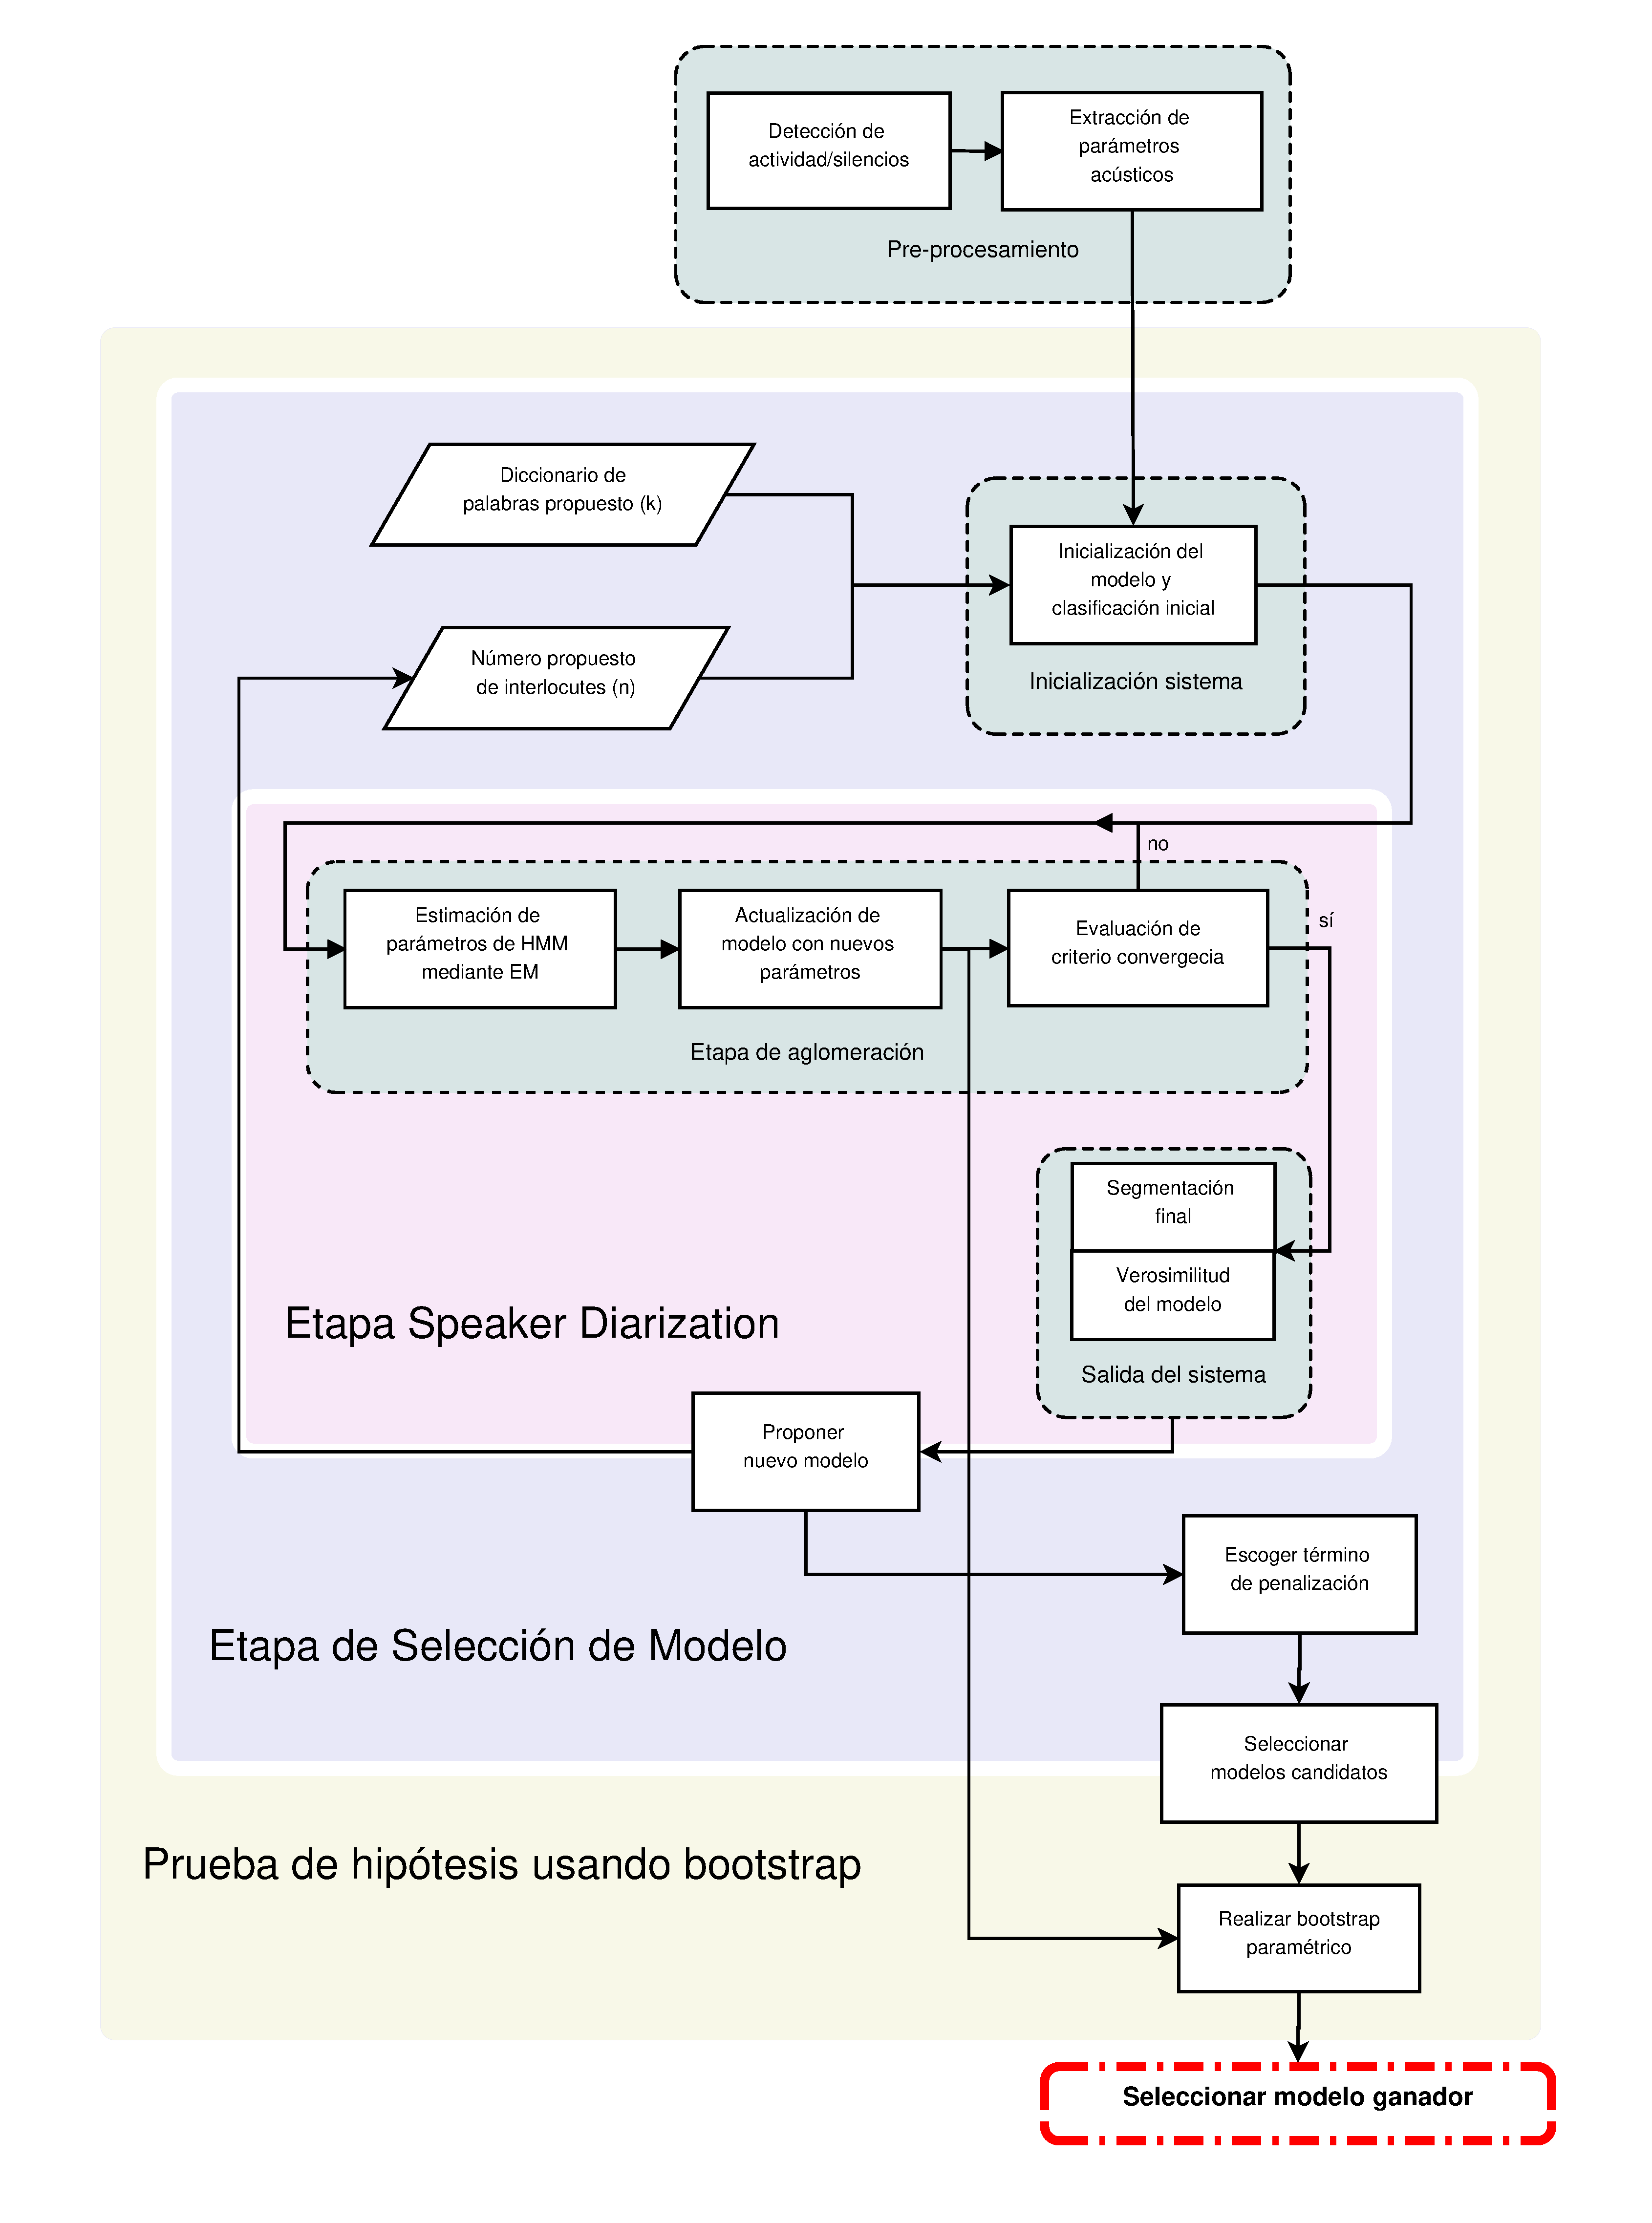
\includegraphics[width=1.5\linewidth]{gfx/chap5/general_flow}} \quad
  \caption{Esquema general.}
  \label{fig:esquema2}
\end{figure}